\documentclass{article}
\usepackage[utf8]{inputenc}

\usepackage{amssymb}
\usepackage{hyperref}
\usepackage{listings}
\usepackage{xcolor}
\usepackage{amsmath}
\usepackage{systeme}
\usepackage{pgfplots}
\usepackage{tikz}
\usepackage{autonum}
\pgfplotsset{compat=1.9}
\usepackage{enumerate}

\definecolor{codegreen}{rgb}{0,0.6,0}
\definecolor{codegray}{rgb}{0.5,0.5,0.5}
\definecolor{codepurple}{rgb}{0.58,0,0.82}
\definecolor{backcolour}{rgb}{0.95,0.95,0.92}

\lstdefinestyle{mystyle}{
    backgroundcolor=\color{backcolour},   
    commentstyle=\color{codegreen},
    keywordstyle=\color{magenta},
    numberstyle=\tiny\color{codegray},
    stringstyle=\color{codepurple},
    basicstyle=\ttfamily\footnotesize,
    breakatwhitespace=false,         
    breaklines=true,                 
    captionpos=b,                    
    keepspaces=true,                 
    numbers=left,                    
    numbersep=5pt,                  
    showspaces=false,                
    showstringspaces=false,
    showtabs=false,                  
    tabsize=2
}

\lstset{style=mystyle}

%Russian-specific packages
%--------------------------------------
\usepackage[T2A]{fontenc}
\usepackage[utf8]{inputenc}
\usepackage[russian]{babel}
%--------------------------------------

\usepackage{geometry}
\geometry{a4paper,left=25mm,top=25mm,bottom=30mm,right=25mm}

\usepackage{indentfirst}
\setlength{\parindent}{2em}

\usepackage{graphicx}
\usepackage{caption}
\graphicspath{ {./img/} }

\usepackage{float}
\usepackage{anyfontsize}

\begin{document}

\begin{titlepage}
      
\end{titlepage}

\begin{titlepage}
	\newgeometry{a4paper,left=20mm,top=20mm,bottom=20mm,right=20mm}
	\begin{center}
	
\includegraphics[height=0.5in]{msu.png}
	\hfill
	\begin{minipage}[b]{0.77\textwidth}
		\centering
		\textbf{\fontsize{12}{9}\selectfont МОСКОВСКИЙ ГОСУДАРСТВЕННЫЙ УНИВЕРСИТЕТ}
		\bigbreak
		\textbf{\fontsize{12}{9}\selectfont имени М.В.Ломоносова}
	\end{minipage}
	\hfill
	
\includegraphics[height=0.5in]{vmk.png}
	\bigbreak
	\textbf{\fontsize{12}{9}\selectfont Факультет вычислительной математики и кибернетики}
	\end{center}
	\vspace{-0.1cm}
	\hrule
	
	\vspace{5cm}
	\begin{center}
	{\fontsize{16}{30}\selectfont 
	\bf Практикум по курсу\\
	"Суперкомпьютеры и параллельная обработка данных"\\
	}
	
	\fontsize{12}{30}\selectfont\bf {Разработка параллельной версии программы для сложения матриц и перемножения векторов
	}
				
	\vspace{2cm}
	
	{\fontsize{16}{30}\selectfont 
	\textbf{ОТЧЕТ\\
	о выполненном задании\\}
	студента 320 учебной группы факультета ВМК МГУ\\
	Грибов Ильи Юрьевича\\}
	\end{center}
	
	\vfill
	\center{Москва\\ 2022}
\end{titlepage}

\tableofcontents

\newpage

\section{Постановка задачи}

\begin{enumerate}
    \item {\large Реализовать алгоритм параллельного подсчета ядра gemver с использованием OpenMP и MPI.}
    \item {\large Исследовать зависимость времени выполнения программы от размера входных данных и числа используемых потоков}.
    \item {\large Построить графики зависимости времени исполнения от числа потоков для различного объёма входных данных}.
    \item {\large Сравнить эффективность OpenMP и MPI-версий параллельной программы.}.
\end{enumerate}

\section{Описание алгоритма и код программы}

{\large Ниже представлена реализация самого наивного алгоритма с использованием вложенных циклов for}.

{\large Математически опишем производимые алгоритмом операции.}
\begin{enumerate}
    \item A = A + $u_1$ * $v_1$ + $u_2$ * $v_2$, где A - это матрица размера n × n, а $u_1$ и $u_2$ - это столбы высоты n, $v_1$ и $v_2$ - это строки длины n.
    \item x = x + \(\beta\) * A * y, где A - это матрица размера n × n , a x и y - это вектор столбцы высоты n, \(\beta\) - вещественный коэффициент.
    \item x = x + z, где x и z - это вектор столбцы высоты n.
    \item w = w + \(\alpha\) * A * x, где A - это матрица размера n × n, a w и x - это вектор столбцы высоты n, \(\alpha\) - вещественный коэффициент.
\end{enumerate}

{\large Ниже представлен код на языке С.}

\vspace{0.5cm}
\begin{lstlisting}[language = C]
        for (int i = 0; i < n; i++) {
            for (int j = 0; j < n; j++) {
                A[i][j] = A[i][j] + u1[i] * v1[j] + u2[i] * v2[j];
            }
        }

        for (int i = 0; i < n; i++) {
            for (int j = 0; j < n; j++) {
                x[i] = x[i] + beta * A[j][i] * y[j];
            }
        }

        for (i = 0; i < n; i++) {
            x[i] = x[i] + z[i];
        }

        for (int i = 0; i < n; i++) {
            for (int j = 0; j < n; j++) {
                w[i] = w[i] + alpha * A[i][j] * x[j];
            }
        }
\end{lstlisting}

{\normalsize Этот алгоритм является итеративным и ориентирован на последовательное вычисление элементов. В худщем случае предполагается выполнение $N\cdot N\cdot N$ операций умножения и сложения элементов матрицы и векторов. Количество выполненных операций имеет порядок O($const\cdot n^3$)}.

\subsection {Параллельный алгоритм}

Для начала обратим внимание на то, что массив А во втором цикле
обходится в неправильном порядке, что в свою очередь не позволяет работать КЭШу. Для того чтобы исрпавить эту проблему было принято решение поменять месатми индексы проходов во 2 цикле. Однако так как цикл, в котором был изменен порядок обхода теперь создает зависимость, на каждом шаге все нити в возможной параллельной области будут одновременно работать с массивом x и на чтение и на запись, было принято решение перейти к блочному выполнению второго цикла.

\vspace{0.5cm}
Экспериментальным путем было выяснено, что для последовательной
программы лучше всего подходит размер блока равный размеру данных, это можно
объяснить большим количеством накладных расходов и большим размером КЭШа на
машине в которой производилась проверка.

\vspace{0.5cm}
Дальнейшая модификация кода сводится к добавлению клаузы \textbf{omp parallel for} и \textbf{pragma omp parallel} в нужных местах.

\subsubsection {OpenMP-версия} 
\vspace{0.5cm}

\begin{lstlisting}[language = C]
    #pragma omp parallel
    {
        int BLOCK_SIZE = n / omp_get_num_threads();
        #pragma omp for
        for (int i = 0; i < n; i++) {
            for (int j = 0; j < n; j++) {
                A[i][j] = A[i][j] + u1[i] * v1[j] + u2[i] * v2[j];
            }
        }

        #pragma omp for
        for (int j1 = 0; j1 < n; j1 += BLOCK_SIZE) {
            for (int i = 0; i < n; ++i) {
                for (int j2 = 0; j2 < min(BLOCK_SIZE, n - j1); ++j2) {
                    x[j1 + j2] = x[j1 + j2] + beta * A[i][j1 + j2] * y[i];
                }
            }
        }

        #pragma omp for
        for (int i = 0; i < n; ++i) {
            x[i] = x[i] + z[i];
        }

        #pragma omp for
        for (int i = 0; i < n; i++) {
            for (int j = 0; j < n; j++) {
                w[i] = w[i] + alpha * A[i][j] * x[j];
            }
        }
    }
\end{lstlisting}
\vspace{0.5cm}

\vspace{0.5cm}
A также при инициализации всех матриц и векторов
\begin{lstlisting}[language = C]
    #pragma omp  parallel for
    for (int i = 0; i < n; i++) {
        u1[i] = i;
        u2[i] = ((i+1)/fn)/2.0;
        v1[i] = ((i+1)/fn)/4.0;
        v2[i] = ((i+1)/fn)/6.0;
        y[i] = ((i+1)/fn)/8.0;
        z[i] = ((i+1)/fn)/9.0;
        x[i] = 0.0;
        w[i] = 0.0;
        for (int j = 0; j < n; j++) {
            A[i][j] = (double) (i*j % n) / n;
        }
    }
\end{lstlisting}
\vspace{0.5cm}

Наиболее важным отличием модифицированного кода перед распаралеливанием является то, что в нем совершенно очевидно можно распределить вычисления в каждом цикле, так как мы четко и ясно избавились от зависимости между нитями, по которым будут разделятся итерации внешнего цикла.

\subsection{MPI-версия}

MPI-версия выглядит следующим образом

\vspace{0.5cm}
В функции void kernel gemver(...)

\begin{lstlisting}[language = C]
    MPI_Status status[1];
    double (*cur)[n]; cur = (double(*)[n])malloc ((n) * sizeof(double));

    int myrank, ranksize;
    MPI_Comm_rank(MPI_COMM_WORLD, &myrank);
    MPI_Comm_size(MPI_COMM_WORLD, &ranksize);

    if (!myrank) {
        for (int j = 0; j < n; j++) {
            x[j] = x[j] + z[j];
        }
        for (int i = 1; i < use_proc; i++) {
            MPI_Recv((*cur), n, MPI_DOUBLE, i, 13, MPI_COMM_WORLD, &status[0]);
            for (int j = 0; j < n; j++) {
                x[j] = x[j] + (*cur)[j];
            }
        }
        for (int i = 1; i < use_proc; i++) {                           //for use * comment it
            MPI_Send(x, n, MPI_DOUBLE, i, 13, MPI_COMM_WORLD);         //for use * comment it
        }                                                              //for use * comment it
    } else {
        MPI_Send(x, n, MPI_DOUBLE, 0, 13, MPI_COMM_WORLD);
        MPI_Recv(x, n, MPI_DOUBLE, 0, 13, MPI_COMM_WORLD, &status[0]); //for use * comment it
    }
    MPI_Bcast(x, n, MPI_DOUBLE, 0, MPI_COMM_WORLD); //*
\end{lstlisting}

\vspace{0.5cm}
В функции main(...)

\begin{lstlisting}[language = C]
    int n = N;
    int myrank, ranksize;

    MPI_Init(&argc, &argv);
    MPI_Comm_rank(MPI_COMM_WORLD, &myrank);
    MPI_Comm_size(MPI_COMM_WORLD, &ranksize);

    use_proc = ranksize;
    int k = n / use_proc;
    int m = n % use_proc;
    if (k == 0) {
        k = 1;
        m = 0;
        use_proc = n;
    }

    for (int i = 0; i < use_proc; i++) {
        if (myrank == i) {
            int start = min(i, m) + i * k;
            int size = k + (i < m);
            int end = start + size;
            MPI_Request req[1];
            MPI_Status status[1];

            double alpha;
            double beta;
            double (*A)[size][n]; A = (double(*)[size][n])malloc ((size) * (n) * sizeof(double));
            double (*u1)[size]; u1 = (double(*)[size])malloc ((size) * sizeof(double));
            double (*v1)[n]; v1 = (double(*)[n])malloc ((n) * sizeof(double));
            double (*u2)[size]; u2 = (double(*)[size])malloc ((size) * sizeof(double));
            double (*v2)[n]; v2 = (double(*)[n])malloc ((n) * sizeof(double));
            double (*w)[size]; w = (double(*)[size])malloc ((size) * sizeof(double));
            double (*x)[n]; x = (double(*)[n])malloc ((n) * sizeof(double));
            double (*y)[size]; y = (double(*)[size])malloc ((size) * sizeof(double));
            double (*z)[n]; z = (double(*)[n])malloc ((n) * sizeof(double));

            init_array (n, size, start, end, &alpha, &beta,
                       *A,
                       *u1,
                       *v1,
                       *u2,
                       *v2,
                       *w,
                       *x,
                       *y,
                       *z);

            double time_1;
            if (myrank == 0) {
                time_1 = MPI_Wtime();
            }

            kernel_gemver (n, size, alpha, beta,
                           *A,
                           *u1,
                           *v1,
                           *u2,
                           *v2,
                           *w,
                           *x,
                           *y,
                           *z);

            if (myrank == 0) {
                size = k + (0 < m);
                for (int k = 0; k < size; k++) {
                    printf("%lf\n", (*w)[k]);
                }
                double (*cur)[size]; cur = (double(*)[size])malloc ((size) * sizeof(double));
                for (int j = 1; j < use_proc; j++) {
                    size = k + (j < m);
                    MPI_Recv(*cur, size, MPI_DOUBLE, j, 13, MPI_COMM_WORLD, &status[0]);
                    for (int k = 0; k < size; k++) {
                        printf("%lf\n", (*cur)[k]);
                    }
                }
                printf("MPI --- %lf\n", MPI_Wtime() - time_1);
            } else {
                MPI_Send(w, size, MPI_DOUBLE, 0, 13, MPI_COMM_WORLD);
            }

            free((void*)A);
            free((void*)u1);
            free((void*)v1);
            free((void*)u2);
            free((void*)v2);
            free((void*)w);
            free((void*)x);
            free((void*)y);
            free((void*)z);
            break;
        }
    }
    MPI_Finalize();
\end{lstlisting}

\section{Тестирование программы}
\subsection{OpenMP}
В этом разделе представлены результаты тестирования, описанных в
предыдущем разделе, программ и трехмерные графики зависимостей. Тестирование
производилось на компьютере Polus.

\vspace{0.5cm}
Конфигурации запущенных программ для OpenMP:
\begin{itemize}
    \item 1, 4, 8, 16, 32, 64 потоков
    \item 40, 120, 400, 2000, 4000, 10000, 20000 размер данных
\end{itemize}

Каждая конфигурация была запущена 5 раз. Ниже приведены усредненные результаты.

\begin{figure}[H]
    \centering
    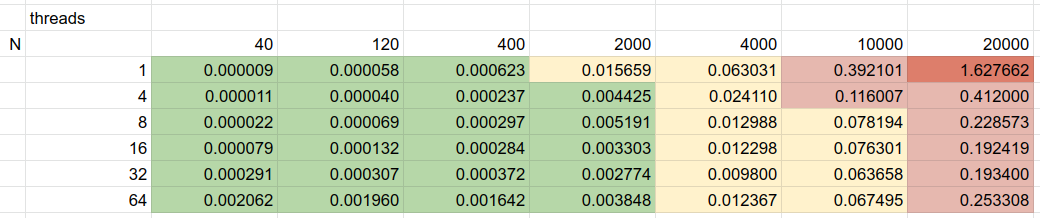
\includegraphics[scale = 0.3]{omp_res.png}
\end{figure}

График, отражающий зависимость времени выполнения программы от различных входных данных и числа процессов.

\begin{figure}[H]
    \centering
    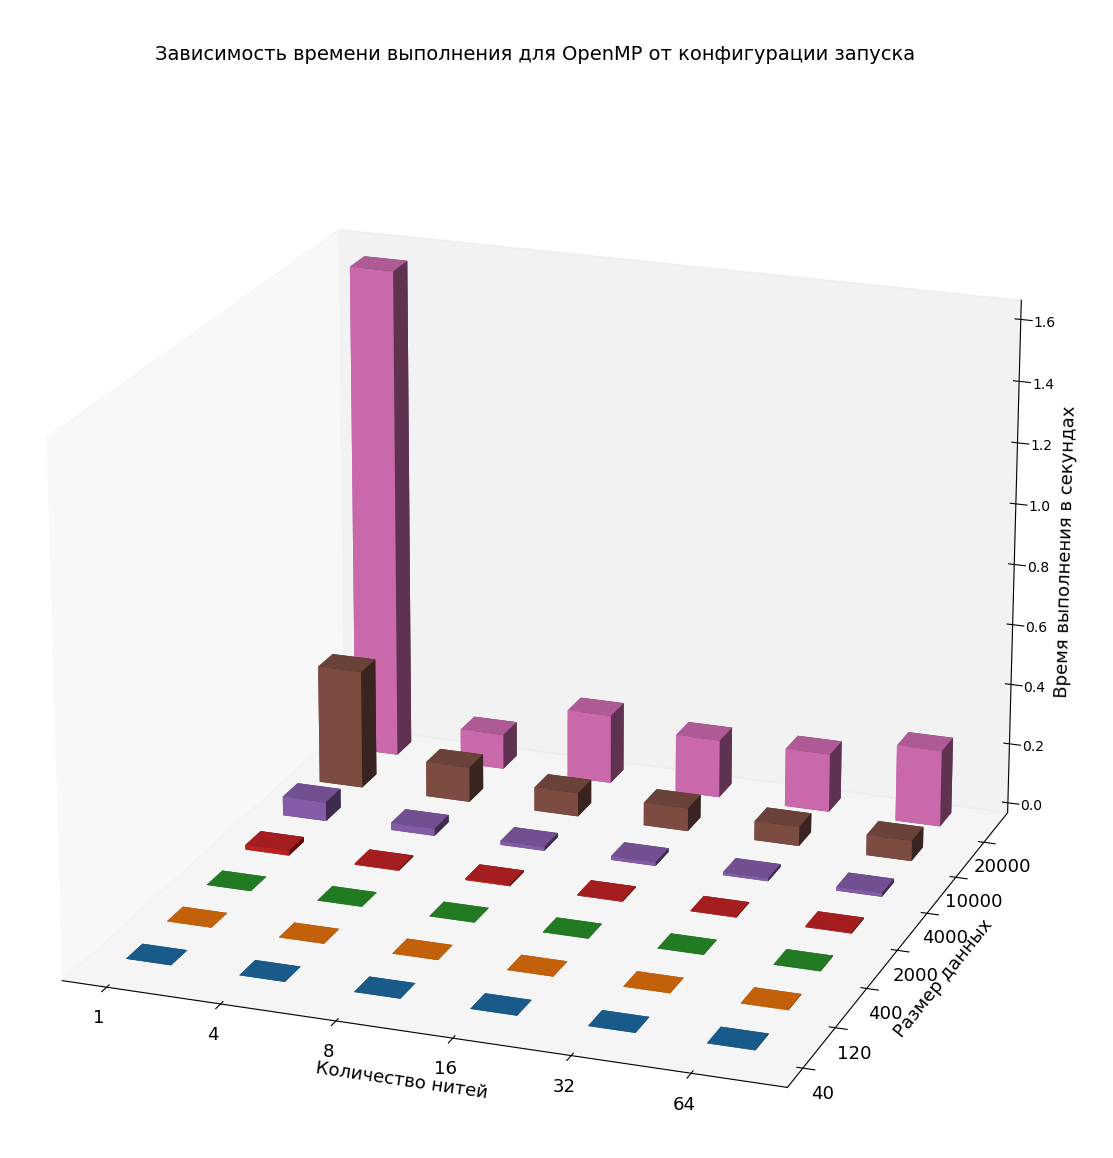
\includegraphics[scale = 0.35,width=15cm,height=13cm]{omp_plot.png}
\end{figure}

\subsection{MPI}

\vspace{0.5cm}
Конфигурации запущенных программ для MPI:
\begin{itemize}
    \item 1, 4, 8, 16, 32, 48 потоков
    \item 40, 120, 400, 2000, 4000, 10000, 20000 размер данных
\end{itemize}

Каждая конфигурация была запущена 5 раз. Ниже приведены усредненные результаты.

\begin{figure}[H]
    \centering
    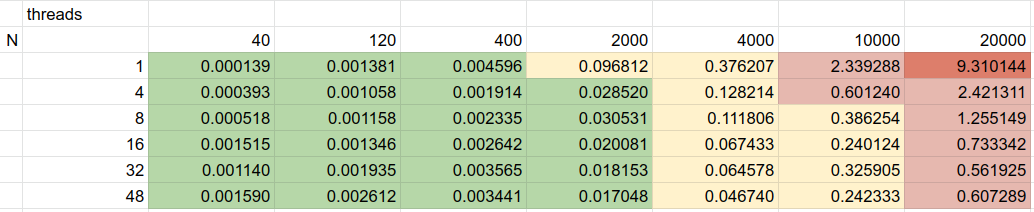
\includegraphics[scale = 0.3]{mpi_res.png}
\end{figure}

График, отражающий зависимость времени выполнения программы от различных входных данных и числа процессов.

\begin{figure}[H]
    \centering
    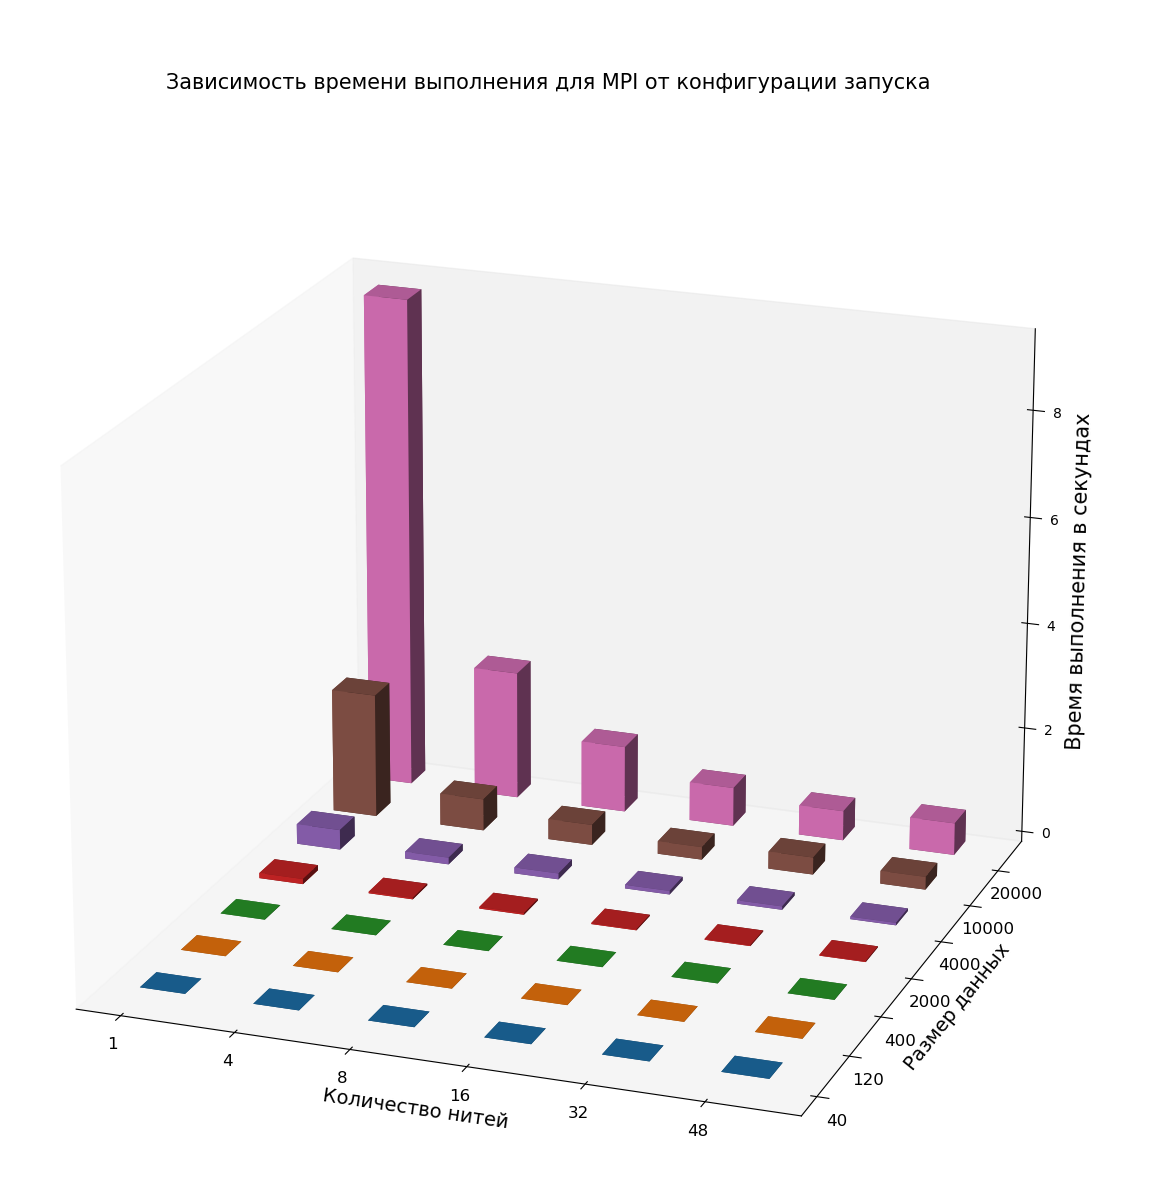
\includegraphics[scale = 0.4,width=16cm,height=16cm]{mpi_plot.png}
\end{figure}

\section{Анализ полученных результатов}

Из проведенных исследований результаты которых приведены в предыдущем
разделе можно сделать множество выводов.
Скорость выполнения программы перестает линейно возрастать в зависимости
от количества потоков на которых выполняется программа по причине того, что
накладные расходы на создание порции нитей значительно увеличиваются, и
проанализировав результаты выполнения можно заметить, что при меньших размерах данных программа перестает ускоряться при меньшем числе потоков. Это
подтверждает идею о том, что накладные расходы на создание нитей - основная
причина недостаточной масщтабируемости программы.

Блочный алгоритм позволяет очень хорошо ускорить программу и избежать
зависимости по данным при параллельном выполнении программы.
Анализируя графики и находя минимумы времени в проекции трехмерного
графика на плоскость с соответствующим размером данных можно установить
оптимальное число потоков для данного размера данных. Например, если
рассматривать Polus и размер данных равный 10000 для MPI, то можно заметить, что минимум времени в проекции трехмерного графика на плоскость соответствующую размеру данных равному 10000 достигается при 32 потоках.

Также из полученных данных видно, что произведенная оптимизация
последовательной программы значительно ускоряет работу и является предельной.

\section{Выводы}
Работа по улучшению и разработке параллельной версии программы при
помощи средств OpenMP позволила значительно ускорить полученную версию
программы и провести ряд экспериментов с таким компьютером как Polus.

OpenMP - это крайне удобная в использовании технология, которая позволяет
быстро получить качественный результат и получить значительный прирост
производительности на различных системах.

\end{document}

